\documentclass{article}

\usepackage[a4paper, margin=0.8in]{geometry}
\usepackage{amsmath}
\usepackage{graphicx}
\usepackage{listings}
\usepackage{xcolor}
\usepackage{float}
\usepackage{placeins}
\usepackage{tikz}

\title{\hspace*{1.5cm}\textbf{EE 341: Communication Systems \newline Assignment 1}}

\author{G\ Raviteja (23110120) \ Govindu Vignesh (23110122)}

\date{}




\lstset{
    language=Matlab,
    basicstyle=\ttfamily\small,
    keywordstyle=\color{blue},
    commentstyle=\color{green!60!black},
    breaklines=true
}
\setlength{\abovedisplayskip}{8pt}
\setlength{\belowdisplayskip}{8pt}

\begin{document}

\maketitle

\section{Identification of AM Variants}

Amplitude Modulation (AM) is one of the fundamental analog modulation techniques used to shift a baseband message signal to a higher carrier frequency for transmission. In AM, the amplitude of the carrier is controlled by the message signal, resulting in spectral components around the carrier frequency. Based on whether the carrier and sidebands are fully transmitted, partially suppressed, or completely removed, several AM variants are obtained, each with distinct spectral characteristics.

Different amplitude modulation variants are identified based on the spectral components present around the carrier frequency.

\begin{itemize}

\item[$\rightarrow$] \textbf{Standard AM (DSB-C):} Carrier and both sidebands are transmitted.

\begin{equation*}
s(t) = A_c \left(1 + \mu m(t)\right)\cos(2\pi f_c t)
\end{equation*}

This produces three spectral components: carrier at $f_c$, upper sideband at $f_c + f_m$, and lower sideband at $f_c - f_m$.

\item[$\rightarrow$] \textbf{DSB-SC (Double Sideband Suppressed Carrier):} Carrier is suppressed and only both sidebands are transmitted.

\begin{equation*}
s(t) = m(t)\cos(2\pi f_c t)
\end{equation*}

This produces two symmetric sidebands around the carrier frequency without a carrier component.

\item[$\rightarrow$] \textbf{SSB (Single Sideband):} Only one sideband is transmitted after suppressing the carrier and one sideband.

Upper sideband:

\begin{equation*}
s_{USB}(t) = A_m \cos\big(2\pi(f_c + f_m)t\big)
\end{equation*}

Lower sideband:

\begin{equation*}
s_{LSB}(t) = A_m \cos\big(2\pi(f_c - f_m)t\big)
\end{equation*}

Only one sideband appears in the spectrum.

\item[$\rightarrow$] \textbf{VSB (Vestigial Sideband):} One sideband is transmitted fully while a partial portion of the other sideband is retained.

\begin{equation*}
s(t) = \text{USB} + \text{partial LSB}
\end{equation*}

This is commonly used where complete sideband suppression is difficult.

\end{itemize}

\subsection*{MATLAB Implementation}

\begin{lstlisting}
clear
clc
close all

% Load the given signal file 
load('A1_Q1_signal.mat')

% Store the signal in a variable
s = s_t;

% Calculate the sampling frequency.
% The sampling interval is the difference between two consecutive time samples
Fs = 1/(t(2) - t(1));

% Find the total number of samples in the signal
N = length(s);

% Compute the Fourier Transform of the signal to convert it
% from time domain to frequency domain
S = fftshift(fft(s));

% Create the corresponding frequency axis for plotting the spectrum
% fftshift places 0 Hz at the center of the spectrum
f = (-N/2 : N/2-1) * (Fs/N);

% Plot the signal in the time domain
figure
plot(t, s)
xlabel('Time (s)')
ylabel('s(t)')
title('Time Domain Signal')
grid on

% Save the time domain plot
saveas(gcf,'st_signal.png')

% Plot the magnitude of the frequency spectrum
figure
plot(f, abs(S))
xlabel('Frequency (Hz)')
ylabel('|S(f)|')
title('Magnitude Spectrum of the Received Signal')
grid on

% Save the spectrum plot
saveas(gcf,'spectrum.png')
\end{lstlisting}

\begin{figure}[H]
\centering

\begin{minipage}{0.40\textwidth}
\centering
\includegraphics[width=\linewidth]{st_signal.png}
\caption{Time-domain representation of the received signal $s(t)$.}
\end{minipage}
\hfill
\begin{minipage}{0.40\textwidth}
\centering
\includegraphics[width=\linewidth]{spectrum.png}
\caption{Magnitude spectrum of the received signal.}
\end{minipage}

\end{figure}

\FloatBarrier


\begin{figure}[H]
\centering
\includegraphics[width=0.7\textwidth]{zoomSpec.png}
\caption{Zoomed Magnitude spectrum}
\end{figure}

\FloatBarrier

\subsection*{Result}

As discussed above, DSB-SC modulation is characterized by suppression of the carrier component while retaining both upper and lower sidebands. The same behavior is evident in the MATLAB-generated frequency spectrum, where symmetric sidebands are observed around the carrier frequency without a dominant spectral peak at the carrier itself. Hence, from the observed spectral structure, \textbf{it can be concluded that the intercepted signal corresponds to DSB-SC modulation}.


\section*{2. Carrier Frequency Estimation}

Since the intercepted signal is identified as a DSB-SC signal, its spectrum contains two dominant sidebands symmetrically located around the carrier frequency. Therefore, the carrier frequency can be estimated by taking the midpoint of the two strongest spectral peaks obtained from the FFT:

\[
f_1 = f_c - f_m, \quad f_2 = f_c + f_m
\]
\[
f_c = \frac{f_1 + f_2}{2}
\]


where $f_1$ and $f_2$ are the frequencies of the two dominant sidebands.
\subsection*{MATLAB Implementation}

\begin{lstlisting}
clear
clc
close all

load('A1_Q1_signal.mat')

s = s_t;
Fs = 1/(t(2)-t(1));
N = length(s);

S = fftshift(fft(s));
f = (-N/2:N/2-1)*(Fs/N);

magS = abs(S);

% keep only positive frequencies
pos_idx = f > 0;
f_pos = f(pos_idx);
mag_pos = magS(pos_idx);

% find two largest peaks in positive spectrum
[~, idx] = maxk(mag_pos,2);

f1 = f_pos(idx(1));
f2 = f_pos(idx(2));

% carrier frequency = midpoint
fc = (f1 + f2)/2;

disp(['Estimated Carrier Frequency: ', num2str(fc), ' Hz'])
\end{lstlisting}

\begin{figure}[H]
\centering
\includegraphics[width=0.55\textwidth]{CarrierFrequency.png}
\caption{Carrier frequency estimation.}
\end{figure}

\FloatBarrier

\subsection*{Result}

The two strongest spectral peaks in the frequency spectrum are centered around $480\text{kHz}$. Hence, the estimated carrier frequency of the intercepted signal is

\begin{equation*}
f_c \approx 480k\ \text{Hz}
\end{equation*}
\section*{3. $\rho$-Occupied Bandwidth}

The $\rho$-occupied bandwidth is the smallest frequency range that contains a fraction $\rho$ of the total signal power. For a signal with spectrum $X(f)$, the total power of the signal in the frequency domain is

\begin{equation}
P_{\text{total}} = \int_{-\infty}^{\infty} |X(f)|^2 \, df .
\end{equation}

Let $f_{\text{peak}}$ be the frequency where the spectrum has its maximum value. We consider a symmetric interval around $f_{\text{peak}}$. The goal is to find the smallest $\Delta f$ such that

\begin{equation}
\frac{\int_{f_{\text{peak}}-\Delta f}^{f_{\text{peak}}+\Delta f} |X(f)|^2 \, df}
{\int_{-\infty}^{\infty} |X(f)|^2 \, df}
\ge \rho .
\end{equation}

The $\rho$-occupied bandwidth is then given by

\begin{equation}
f_{BW}(\rho) = 2\Delta f^* .
\end{equation}

In practice, the FFT of the signal is first computed to obtain the power spectrum $|X(f)|^2$. Since the signal is real, the spectrum is symmetric, so only the positive frequencies are used. The spectral peak $f_{\text{peak}}$ is found as the frequency with the maximum power. Starting from this peak, the frequency interval is slowly expanded on both sides by including neighbouring frequency points. At each step, the power inside this interval is added and compared with the total signal power. The expansion continues until the collected power becomes greater than or equal to the required fraction $\rho$ of the total power. The width of this interval is then taken as the $\rho$-occupied bandwidth.

\subsection*{MATLAB Implementation}

\begin{lstlisting}
clear
clc
close all

load('A1_Q1_signal.mat')

s = s_t;
time = t;

Fs = 1/(time(2)-time(1));
N = length(s);

S = fftshift(fft(s));
f = linspace(-Fs/2, Fs/2, N);

% compute power spectrum |X(f)|^2 from FFT
P = abs(S).^2;

% keep only positive frequencies since spectrum is symmetric for real signals
pos = f > 0;
f = f(pos);
P = P(pos);

% total signal power (denominator in the rho condition)
P_total = sum(P);

% find spectral peak frequency f_peak
[~, peak_idx] = max(P);
f_peak = f(peak_idx);

rho_values = [0.9 0.95 0.99 0.999 0.9999];
BW = zeros(size(rho_values));

for r = 1:length(rho_values)

    rho = rho_values(r);

    % start interval at the spectral peak
    left = peak_idx;
    right = peak_idx;

    % power currently captured inside the interval
    power_sum = P(peak_idx);

    % expand interval symmetrically around f_peak
    % until the captured power fraction reaches rho
    while power_sum/P_total < rho && left>1 && right<length(P)

        left = left - 1;
        right = right + 1;

        % add power from the new frequency bins
        power_sum = power_sum + P(left) + P(right);

    end

    % occupied bandwidth = width of the interval around the peak
    BW(r) = f(right) - f(left);

end

fprintf('Spectral Peak Frequency = %.2f Hz\n\n', f_peak);

for i = 1:length(rho_values)
    fprintf('rho = %.4f  -->  Occupied Bandwidth = %.2f Hz\n', rho_values(i), BW(i));
end
\end{lstlisting}

\begin{figure}[H]
\centering
\includegraphics[width=0.55\textwidth]{q3.png}
\caption{Occupied Bandwidth}
\end{figure}

\FloatBarrier

\subsection*{Results}

The spectral peak of the intercepted signal was first identified from the power spectrum. The peak frequency was found to be

\begin{equation}
f_{\text{peak}} = 480056.78 \ \text{Hz}.
\end{equation}

Using this peak as the center frequency, the $\rho$-occupied bandwidth was computed for different values of $\rho$. The obtained results are shown below:

\begin{center}
\begin{tabular}{c c}
\hline
$\rho$ & Occupied Bandwidth (Hz) \\
\hline
0.90   & 1596.54 \\
0.95   & 5949.39 \\
0.99   & 12045.72 \\
0.999  & 21238.46 \\
0.9999 & 28893.99 \\
\hline
\end{tabular}
\end{center}

From the results, it can be observed that the occupied bandwidth increases as $\rho$ increases. This happens because a larger value of $\rho$ requires that a larger portion of the total signal power be captured, which requires expanding the frequency interval around the spectral peak.

\section*{4. Number of Audio Channels}


To determine the number of audio channels present in the signal, the frequency spectrum around the carrier frequency is examined.

Each audio channel that modulates the carrier produces two sidebands around the carrier frequency. Therefore, the number of channels can be estimated by observing the number of distinct bands present in the magnitude spectrum.

In practice, the received signal may contain noise and spectral leakage due to the finite observation window. These effects can create additional small peaks near the actual signal components. Hence, the spectrum is visually inspected and the number of clear bands around the carrier frequency is counted. Each pair of bands corresponds to one audio channel.

\subsection*{MATLAB Implementation}

\begin{lstlisting}
clear
clc
close all
load('A1_Q1_signal.mat')

s = s_t;
Fs = 1/(t(2)-t(1));
N = length(s);

% Compute spectrumS
S = fftshift(fft(s));
f = (-N/2:N/2-1)*(Fs/N);

% Plot zoomed spectrum around carrier
figure
plot(f,abs(S))
xlim([478000 482000])   % zoom around carrier region
xlabel('Frequency (Hz)')
ylabel('|S(f)|')
title('Zoomed Spectrum Around Carrier')
grid on

saveas(gcf,'AudioChannels.png')
\end{lstlisting}

\begin{figure}[H]
\centering
\includegraphics[width=0.55\textwidth]{AudioChannels.png}
\caption{Zoomed spectrum around the carrier showing the modulated bands.}
\end{figure}

\FloatBarrier

\subsection*{Results}

From the magnitude spectrum of the intercepted signal, two clear bands are observed around the carrier frequency. These two bands correspond to the sidebands of a single modulated signal.

Hence, the intercepted signal contains \textbf{one audio channel}.
\section*{5. Receiver Design for Extracting an Audio Channel}

Since the intercepted signal has been identified as a \textbf{DSB-SC signal}, coherent demodulation is required for message recovery because the carrier component is suppressed and envelope detection cannot recover the message correctly.

The received signal can be expressed as

\begin{equation*}
r(t)=m(t)\cos(2\pi f_c t)
\end{equation*}
\vspace{-0.3cm}

At the receiver, a locally generated carrier synchronized to the estimated carrier frequency is multiplied with the received signal:

\begin{equation*}
r_{mix}(t)=r(t)\cos(2\pi f_c t)
\end{equation*}
\vspace{-0.3cm}

Using the trigonometric identity $\cos A \cos B = \frac{1}{2}[\cos(A-B)+\cos(A+B)]$, the mixer output becomes

\begin{equation*}
r_{mix}(t)=\frac{m(t)}{2}+\frac{m(t)}{2}\cos(4\pi f_c t)
\end{equation*}
\vspace{-0.3cm}

Thus, the output contains:

\begin{itemize}
\item[$\rightarrow$] Desired baseband message term $\frac{m(t)}{2}$
\item[$\rightarrow$] High-frequency component centered at $2f_c$
\end{itemize}

To recover the message, a low-pass filter is applied to remove the high-frequency term.
\newpage

\subsection*{Receiver Block Diagram}

\begin{center}
Received Signal $\rightarrow$ Mixer $\times \cos(2\pi f_c t)$ $\rightarrow$ Low Pass Filter $\rightarrow$ Recovered Audio
\end{center}

\begin{figure}[h]
\centering
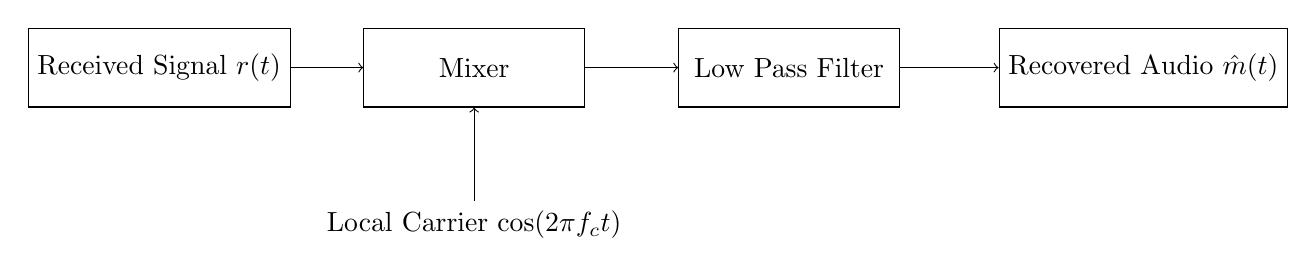
\begin{tikzpicture}[node distance=2cm, auto]

\node [draw, rectangle, minimum width=2.8cm, minimum height=1cm] (rx) {Received Signal $r(t)$};

\node [draw, rectangle, minimum width=2.8cm, minimum height=1cm, right of=rx, node distance=4cm] (mixer) {Mixer};

\node [draw, rectangle, minimum width=2.8cm, minimum height=1cm, right of=mixer, node distance=4cm] (lpf) {Low Pass Filter};

\node [draw, rectangle, minimum width=3cm, minimum height=1cm, right of=lpf, node distance=4.5cm] (out) {Recovered Audio $\hat{m}(t)$};

\node [below of=mixer, node distance=2cm] (carrier) {Local Carrier $\cos(2\pi f_c t)$};

\draw[->] (rx) -- (mixer);
\draw[->] (mixer) -- (lpf);
\draw[->] (lpf) -- (out);
\draw[->] (carrier) -- (mixer);

\end{tikzpicture}
\caption{Coherent receiver structure used for DSB-SC demodulation}
\end{figure}


\subsection*{Low-Pass Filter Design}

The cutoff frequency of the low-pass filter is selected using the occupied bandwidth obtained in Question 3 so that nearly all message power is preserved while rejecting the component around $2f_c$ generated after coherent multiplication.

For the present signal,

\begin{equation*}
f_{BW}(0.9999) \approx 28893,\text{Hz} \approx 30\text{kHz}
\end{equation*}
\vspace{-0.3cm}

Since a DSB-SC signal contains symmetric upper and lower sidebands, the corresponding baseband bandwidth is approximately half of the total occupied bandwidth. Therefore, the low-pass filter cutoff is chosen as

\begin{equation*}
f_{LPF} \approx \frac{f_{BW}(0.9999)}{2} \approx 15\text{kHz}
\end{equation*}
\vspace{-0.3cm}

This ensures that the message signal is retained while the high-frequency term produced during demodulation is effectively removed.


\subsection*{MATLAB Implementation}

\begin{lstlisting}
clear
clc
close all

load('A1_Q1_signal.mat')
s = s_t;
Fs = 1/(t(2)-t(1));
fc = 480000;

% Generate local carrier
carrier = cos(2*pi*fc*t);

% Coherent demodulation
demod_signal = s .* carrier;

% Low-pass filter to recover audio
audio = lowpass(demod_signal,15000,Fs);

%% Time-domain plot
figure
plot(t,audio)
xlabel('Time (s)')
ylabel('Amplitude')
title('Recovered Audio Signal (Time Domain)')
grid on
saveas(gcf,'RecoveredAudio_Time.png')

%% Frequency-domain plot
N = length(audio);
A = fftshift(fft(audio));
f = (-N/2:N/2-1)*(Fs/N);

figure
plot(f,abs(A))
xlabel('Frequency (Hz)')
ylabel('Magnitude')
title('Recovered Audio Signal (Frequency Domain)')
xlim([-20000 20000])
grid on
saveas(gcf,'RecoveredAudio_Freq.png')
\end{lstlisting}

\begin{figure}[H]
\centering

\begin{minipage}{0.48\textwidth}
\centering
\includegraphics[width=\linewidth]{RecoveredAudio_Time.png}
\caption{Recovered audio signal in time domain}
\end{minipage}
\hfill
\begin{minipage}{0.48\textwidth}
\centering
\includegraphics[width=\linewidth]{RecoveredAudio_Freq.png}
\caption{Recovered audio signal in frequency domain}
\end{minipage}

\end{figure}


\subsection*{Result}
 The coherent receiver designed successfully recovers the baseband message signal from the intercepted DSB-SC waveform. The low-pass filter removes the high-frequency component and preserves the useful audio content.


\section*{6. Audio Signal Playback}

After recovering the baseband signal using coherent demodulation, the output still remains sampled at the original intercept sampling frequency, which is much higher than the actual audio bandwidth. Direct playback at this sampling rate produces distorted or slow audio because the signal contains far more samples than required for standard audio reproduction.

To obtain correct playback, the demodulated signal is first low-pass filtered and then decimated to a standard audio sampling rate. Decimation reduces the number of samples while preserving the useful message content.

If the original sampling frequency is $F_s$, and the desired audio playback sampling rate is $F_{audio}$, the decimation factor is chosen as

\begin{equation*}
D = \text{round}\left(\frac{F_s}{F_{audio}}\right)
\end{equation*}
\vspace{-0.3cm}

The new playback sampling frequency becomes

\begin{equation*}
F_{new} = \frac{F_s}{D}
\end{equation*}
\vspace{-0.3cm}

A standard audio rate of $44.1\text{kHz}$ is selected because it provides natural playback and preserves the recovered speech content.

\newpage
\subsection*{MATLAB Implementation}

\begin{lstlisting}

clear
clc
close all

load('A1_Q1_signal.mat')
s = s_t;
Fs = 1/(t(2)-t(1));
fc = 480000;

% Generate local carrier
carrier = cos(2*pi*fc*t);

% Coherent demodulation
demod_signal = s .* carrier;

% Low-pass filter
audio = lowpass(demod_signal,15000,Fs);

% Normalize
audio = audio / max(abs(audio));

% Desired audio sampling frequency
Fs_audio = 44100;

% Decimation factor
D = round(Fs/Fs_audio);

% Decimate signal
audio_dec = decimate(audio,D);

% New sampling frequency
Fs_new = Fs/D;

% Normalize again
audio_dec = audio_dec / max(abs(audio_dec));

% Play audio
soundsc(audio_dec, Fs_new);

% Save audio file
audiowrite('RecoveredAudio.wav', audio_dec, Fs_new);


\end{lstlisting}

\subsection*{Result}

After applying decimation and playback at the adjusted sampling frequency, the recovered signal contains a clearly audible rock band audio recording. This verifies that the demodulated signal has been correctly converted into a standard audio format without significant distortion.
\end{document}